\chapter{Analisi di Dati Temporali}

La neccessit{\`a} di trarre conclusioni incrementali per quanto riguarda i dati presenti in uno stream spesso non {\`e} soddisfacibile. Sebbene l'idea chiave risulti ancora oggi abbastanza vincente, tuttavia, la ricorsivit{\`a} non {\`e} caratteristica comune a tutti i problemi che si vorrebbero affrontare sui dati provenienti da uno stream: molti problemi hanno bisogno di processare necessariamente un insieme di dati per volta, con le dovute complicazioni in termini di consumi e performance.

La letteratura ha fornito diversi esempi di modelli per l'analisi progressiva dei data stream, probabilmente quello pi{\`u} vincente {\`e} sicuramente il modello basato sulle finestre temporali (time windows).

Una finestra temporale {\`e}, intuitivamente, una partizione dell'asse temporale, di ampiezza fissa o variabile, a partire da un determinato punto temporale.

\begin{defn}
Si definisce finestra temporale $W(t,\Delta t)$, che comincia all'istante \( t \) con un'ampiezza $\Delta t$, come l'intervallo di tempo intercorrente fra l'istante \( t \) e l'istante $t+\Delta t$.
\end{defn}

La finestra temporale, appena definita in accezione puramente temporale, solitamente sottende una partizione sui dati in ingresso che sono time-stamped. Se, ad esempio, avessimo un data stream caratterizzato alla maniera seguente:

\begin{equation}
DS = \lbrace (d_1,t_1),(d_2,t_2),(d_3,t_3),(d_4,t_4),(d_5,t_5) \rbrace
\end{equation}
 
ossia un data stream che ha ricevuto soltanto 5 dati \( (d_i) \) in altrettanti istanti temporali \( (t_i) \) differenti, allora la finestra temporale \( W(2,2) \) risulta essere come segue:

\begin{equation}
W(2,2) = \lbrace(d_2,t_2),(d_3,t_3)\rbrace
\end{equation}

{\`E} facile capire come $W(t,\Delta t)$ induca sempre l'individuazione di un sottinsieme di \( DS \); occorre pertanto dare una definizione operativa di finestra temporale in funzione di un data stream associato.

\begin{defn}
Si definisce finestra temporale associata al data sream \( DS \), a partire dall'istante \( t \) con un'ampiezza $\Delta t$, come il sottinsieme dei dati presenti nel data stream il cui istante di arrivo {\`e} compreso nell'intervallo $[t,\Delta t]$

\begin{equation}
W(DS,t,\Delta t) = \lbrace (d_i,t_i) \in DS \mid t_i \in [t,\Delta t]\rbrace
\end{equation}
\end{defn}

In quest'ottica operativa vale sempre la propriet{\`a} secondo cui \\ $W(DS,t,\Delta t) \subseteq DS$.

Questa definizione generale di finestra temporale, in realt{\`a}, nasconde tutta una serie di modelli di finestre temporali derivate a partire dal concetto base.

Esistono modelli che consentono ad alcune delle variabili indipendenti $(DS,t,\Delta t)$ di variare nel tempo: una finestra temporale infatti, a seconda del modello considerato, pu{\`o} traslare in avanti nel tempo, variare la propria ampiezza o addirittura fare entrambe le cose.

\section{Landmark Windows}

Il modello temporale di tipo landmark afferisce ad una particolare tipologia di finestre temporali $W(DS,t,\Delta t)$ in cui il parametro di ampiezza $\Delta t$ pu{\`o} aumentare nel tempo. Questo tipo di finestra temporale ha la particolare inefficienza di crescere di dimensione nel tempo ($\Omega(\Delta t)$ dati dove $\Delta t$ {\`e} l'ampiezza iniziale), se non limitata, rendendo potenzialmente inefficiente (in base alla quantit{\`a} di dati esibiti) qualsiasi algoritmo che non scala in maniera adeguata.

\begin{figure}\centering
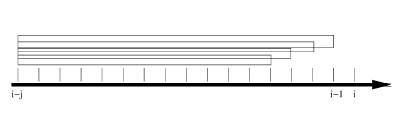
\includegraphics[scale=0.70]{img/landmark-windows}
\caption{Una landmark window che cresce fino all'instante temporale \( i-1 \).}
\end{figure}

Le finestre temporali di tipo landmark, tuttavia, hanno provato la loro efficacia nel risolvere quei problemi incrementali, specie in quelli dove c'{\`e} un uso abbondante di ``blocking operations" oltre ad un'assenza di ricorsivit{\`a}. 

Ai fini della tesi in esame, questa finestra temporale crescente nel tempo riveste un interesse particolare in quanto ci permetter{\`a} di adempiere agli obbiettivi prefissati, ossia quello di investigare lo studio dei cambiamenti della comunit{\`a} per caratterizzare l'evoluzione attraverso la scopera di interazioni tra i partecipanti.

% \section{Grafo Temporale}


% \subsection{Grafo Temporale Cumulativo}

% \begin{figure}\centering
% 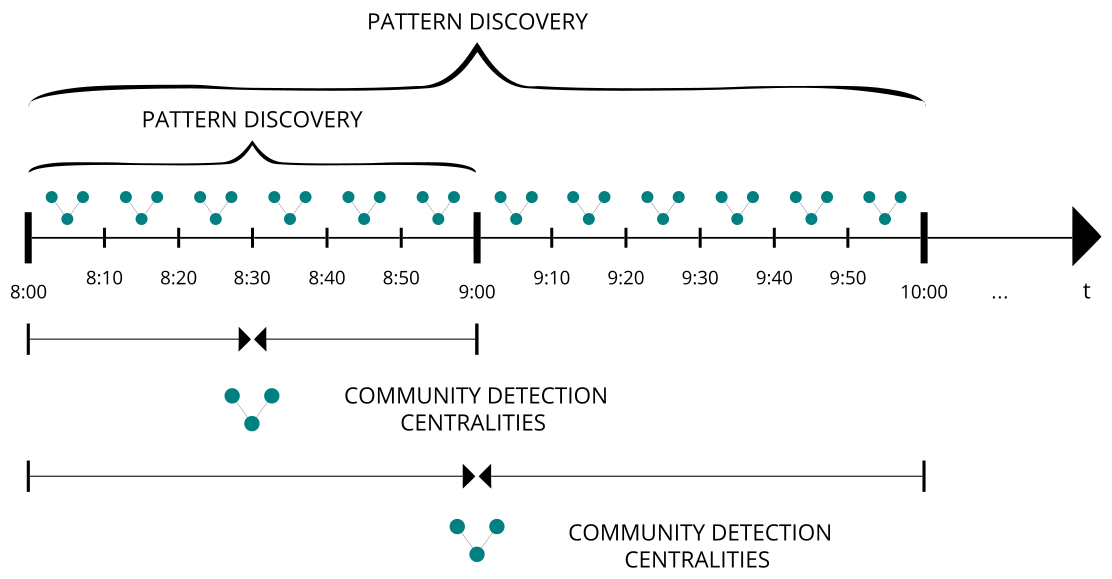
\includegraphics[scale=0.30]{img/temp-graph}
% \caption{.}
% \end{figure}